\documentclass[10pt,twocolumn,letterpaper]{article}
% Layout modelled on the REVTeX 4.2 two-column preprint style (Palatino text, centred small-caps
% section heads, "FIG." captions), built with standard packages.
\usepackage[T1]{fontenc}
\usepackage[sc]{mathpazo}
\linespread{1.04}
\usepackage[letterpaper,top=0.85in,bottom=0.9in,left=0.72in,right=0.72in,columnsep=0.28in]{geometry}
\usepackage{amsmath,amssymb}
\usepackage{graphicx}
\usepackage{booktabs}
\usepackage{xcolor}
\usepackage{microtype}
\usepackage{titlesec}
\usepackage{fancyhdr}
\usepackage[labelsep=colon,font=small,justification=justified,singlelinecheck=true]{caption}
\usepackage[sort&compress,numbers]{natbib}
\usepackage[colorlinks=true,linkcolor=blue!55!black,citecolor=blue!55!black,urlcolor=blue!55!black]{hyperref}
\usepackage{url}
\usepackage{orcidlink}
\usepackage{enumitem}
\usepackage[section]{placeins}
\renewcommand{\topfraction}{0.9}\renewcommand{\bottomfraction}{0.8}\renewcommand{\textfraction}{0.07}\renewcommand{\floatpagefraction}{0.75}\renewcommand{\dbltopfraction}{0.9}\renewcommand{\dblfloatpagefraction}{0.75}
\setlist{nosep,leftmargin=1.2em}

% generated by make_tex_inputs.py from paper_stats.json -- do not edit
\newcommand{\NCounties}{3{,}144}
\newcommand{\NMetro}{1{,}164}
\newcommand{\NRural}{1{,}563}
\newcommand{\NFrontier}{417}
\newcommand{\BirthsTotal}{3{,}642{,}063}
\newcommand{\NFallback}{48}
\newcommand{\NFallbackSupp}{39}
\newcommand{\NPlacesPrior}{187}
\newcommand{\NSmallBirths}{97}
\newcommand{\FTUnique}{26{,}642}
\newcommand{\FTRaw}{27{,}506}
\newcommand{\FTLocations}{18{,}908}
\newcommand{\FTPPW}{4{,}600}
\newcommand{\FTPPWPlaced}{4{,}585}
\newcommand{\FTPPWLoc}{4{,}516}
\newcommand{\FTAssignedPct}{99.7}
\newcommand{\FTUnassigned}{85}
\newcommand{\FTMismatch}{10}
\newcommand{\FTMH}{12{,}637}
\newcommand{\FTSA}{12{,}047}
\newcommand{\FTOTP}{1{,}958}
\newcommand{\ShareSAPPW}{38.2}
\newcommand{\PPWMedicaid}{87.2}
\newcommand{\PPWMOUD}{78.2}
\newcommand{\PPWChildcare}{7.9}
\newcommand{\PPWResbeds}{4.3}
\newcommand{\HCSites}{11{,}769}
\newcommand{\HCLocations}{11{,}219}
\newcommand{\HCUnplaced}{58}
\newcommand{\Clinicians}{1{,}544{,}251}
\newcommand{\OBTotal}{82{,}517}
\newcommand{\BHPTotal}{122{,}193}
\newcommand{\BHTTotal}{1{,}184{,}102}
\newcommand{\FMTotal}{155{,}439}
\newcommand{\NNoPPW}{1{,}793}
\newcommand{\PctNoPPW}{57.0}
\newcommand{\PctBirthsNoPPW}{12.7}
\newcommand{\BirthsNoPPW}{461{,}220}
\newcommand{\NNoBHP}{905}
\newcommand{\NNoOB}{1{,}088}
\newcommand{\NNoHC}{969}
\newcommand{\NNoAny}{604}
\newcommand{\BirthsNoAny}{50{,}457}
\newcommand{\NHNLC}{107}
\newcommand{\HNLCRural}{72}
\newcommand{\HNLCFrontier}{12}
\newcommand{\HNLCMetro}{23}
\newcommand{\HNLCNonmetro}{83}
\newcommand{\KWH}{182.6}
\newcommand{\KWp}{<10^{-39}}
\newcommand{\ChiSq}{423.9}
\newcommand{\Chip}{<10^{-92}}
\newcommand{\RhoNeedCap}{0.24}
\newcommand{\RhoNeedCapp}{<10^{-41}}
\newcommand{\RhoDepSVI}{0.04}
\newcommand{\RhoDepCap}{0.19}
\newcommand{\RhoSVICap}{0.18}
\newcommand{\NeedMedNoPPW}{48.8}
\newcommand{\NeedMedPPW}{54.8}
\newcommand{\MWp}{<10^{-14}}
\newcommand{\CapMedSmall}{21.4}
\newcommand{\CapMedBig}{67.3}
\newcommand{\NBirthsBig}{365}
\newcommand{\ValROB}{0.93}
\newcommand{\ValRPsy}{0.89}
\newcommand{\ValRhoOB}{0.86}
\newcommand{\ValRhoPsy}{0.79}
\newcommand{\ValN}{3{,}135}
\newcommand{\ValSumOBN}{81{,}410}
\newcommand{\ValSumOBA}{43{,}842}
\newcommand{\ValSumPsyN}{119{,}808}
\newcommand{\ValSumPsyA}{37{,}617}
\newcommand{\ValZeroOB}{80.0}
\newcommand{\ValZeroPsy}{69.1}
\newcommand{\StateMinPPW}{4.5}
\newcommand{\StateMinPPWst}{TX}
\newcommand{\StateMaxPPW}{43.8}
\newcommand{\StateMaxPPWst}{VT}
\newcommand{\StateMedPPW}{14.8}
\newcommand{\NStatesHNLC}{22}
\newcommand{\NVBirths}{32{,}888}
\newcommand{\NVNoPPW}{10}
\newcommand{\NVFrontier}{11}
\newcommand{\NVPPW}{42}
\newcommand{\NVPctBirthsNoPPW}{2.5}
\newcommand{\NVNoOB}{7}
\newcommand{\NVNoBHP}{5}
\newcommand{\NVCWBirths}{89.9}
\newcommand{\NVCWPPW}{69.0}
\newcommand{\ROB}{0.925}
\newcommand{\NoPPWMetro}{35.1}
\newcommand{\NoBHPMetro}{11.2}
\newcommand{\NoOBMetro}{16.5}
\newcommand{\NoHCMetro}{18.6}
\newcommand{\GapMedMetro}{-7.9}
\newcommand{\NeedMedMetro}{49.5}
\newcommand{\CapMedMetro}{58.8}
\newcommand{\DepMedMetro}{23.2}
\newcommand{\SVIMedMetro}{0.47}
\newcommand{\PctBirthsMetro}{86.6}
\newcommand{\BirthsNoPPWMetro}{211{,}647}
\newcommand{\BHPerKMetro}{219.5}
\newcommand{\OBPerKMetro}{14.3}
\newcommand{\NoPPWRural}{65.5}
\newcommand{\NoBHPRural}{30.3}
\newcommand{\NoOBRural}{36.7}
\newcommand{\NoHCRural}{30.6}
\newcommand{\GapMedRural}{6.9}
\newcommand{\NeedMedRural}{56.5}
\newcommand{\CapMedRural}{47.7}
\newcommand{\DepMedRural}{23.5}
\newcommand{\SVIMedRural}{0.56}
\newcommand{\PctBirthsRural}{12.7}
\newcommand{\BirthsNoPPWRural}{231{,}188}
\newcommand{\BHPerKRural}{127.8}
\newcommand{\OBPerKRural}{6.8}
\newcommand{\NoPPWFrontier}{86.6}
\newcommand{\NoBHPFrontier}{72.4}
\newcommand{\NoOBFrontier}{77.2}
\newcommand{\NoHCFrontier}{65.9}
\newcommand{\GapMedFrontier}{-1.6}
\newcommand{\NeedMedFrontier}{35.6}
\newcommand{\CapMedFrontier}{33.8}
\newcommand{\DepMedFrontier}{20.9}
\newcommand{\SVIMedFrontier}{0.34}
\newcommand{\PctBirthsFrontier}{0.8}
\newcommand{\BirthsNoPPWFrontier}{18{,}385}
\newcommand{\BHPerKFrontier}{70.0}
\newcommand{\OBPerKFrontier}{0.0}
\newcommand{\TopStates}{MS (60.9\%), SD (46.8\%), NE (39.1\%), AR (36.0\%), MO (35.3\%)}
\newcommand{\ZeroStates}{CT, DC, DE, HI}
\newcommand{\HNLCStates}{TN (22), TX (21), KY (10), AR (8), AL (7)}
\newcommand{\SensRhoMin}{0.973}
\newcommand{\SensJacMin}{0.59}
\newcommand{\SensWomenRho}{0.994}
\newcommand{\SensWomenStorey}{-63.5}
\newcommand{\SensUnrankedJac}{0.87}
\newcommand{\SensUnrankedN}{110}


\DeclareCaptionLabelFormat{revfig}{FIG.~#2}
\DeclareCaptionLabelFormat{revtab}{TABLE~#2}
\captionsetup[figure]{labelformat=revfig}
\captionsetup[table]{labelformat=revtab,position=top}
\renewcommand{\thetable}{\Roman{table}}

\titleformat{\section}{\centering\normalfont\small\bfseries}{\Roman{section}.}{0.6em}{\MakeUppercase}
\titlespacing*{\section}{0pt}{1.4ex plus .4ex}{0.9ex}
\titleformat{\subsection}{\centering\normalfont\small\bfseries}{\Alph{subsection}.}{0.5em}{}
\titlespacing*{\subsection}{0pt}{1.2ex plus .3ex}{0.7ex}
\titleformat{\subsubsection}[runin]{\normalfont\small\itshape}{\arabic{subsubsection}.}{0.4em}{}[.]
\titlespacing*{\subsubsection}{\parindent}{0.8ex}{0.6em}

\pagestyle{fancy}\fancyhf{}\fancyhead[R]{\small\thepage}\renewcommand{\headrulewidth}{0pt}
\fancypagestyle{plain}{\fancyhf{}\renewcommand{\headrulewidth}{0pt}}
\setlength{\parindent}{1.2em}
\setlength{\bibsep}{1.2pt}
\renewcommand{\bibfont}{\footnotesize}
\renewcommand{\refname}{References}

\begin{document}

\twocolumn[
\begin{@twocolumnfalse}
\begin{center}
{\large\bfseries Where Perinatal Behavioral Health Need Outpaces Treatment Capacity:\\[2pt]
An Open County-Level Need and Capacity Panel for the United States\par}
\vspace{8pt}
{\normalsize Munachimso A. Emesobum\,\orcidlink{0009-0002-7506-2153}\,\textsuperscript{1,\,$*$}\par}
\vspace{3pt}
{\small\itshape \textsuperscript{1}Independent Researcher, Nevada, USA\par}
\vspace{10pt}
\begin{minipage}{0.80\textwidth}
\small
Mental health conditions, including substance use disorders, are a leading underlying cause of pregnancy-related death in the United States, yet agencies deciding where to add perinatal screening, referral, and treatment have had no open national table that sets county need beside county treatment capacity. We built the U.S. County Perinatal Behavioral Health Need and Capacity Panel, a versioned, fully reproducible county-level dataset for all \NCounties\ counties and county-equivalents of the 50 states and the District of Columbia, assembled only from open federal sources. Need is described by births (NCHS natality via the Area Health Resources Files), women aged 15--44, model-based adult depression prevalence (CDC PLACES), and the CDC/ATSDR Social Vulnerability Index. Capacity is described by \FTUnique\ SAMHSA FindTreatment.gov treatment listings (\FTAssignedPct\% placed in a county) coded for pregnant/postpartum (PPW) programs, \HCSites\ HRSA health center sites, and \Clinicians\ obstetric, behavioral health, and family medicine clinicians identified by NUCC taxonomy codes in the CMS NPPES registry. Each county receives percentile-based need and capacity scores, a need-minus-capacity gap score, rural and frontier flags, data-year fields, and small-number flags. We find that \NNoPPW\ counties (\PctNoPPW\%), home to \PctBirthsNoPPW\% of U.S. births, have no substance use treatment listing with a PPW program; the share rises from \NoPPWMetro\% of metro to \NoPPWRural\% of rural and \NoPPWFrontier\% of frontier counties. The PPW program field exists only for substance use listings, so open data cannot identify perinatal-specific mental health facilities. Need and capacity are only weakly related across counties (Spearman $\rho=\RhoNeedCap$), and \NHNLC\ counties combine top-quartile need with bottom-quartile capacity, \HNLCRural\ of them rural. Clinician counts agree closely with independent AMA-based counts (log-scale $r=\ValROB$ obstetric, $\ValRPsy$ psychiatric), and gap rankings are robust to eight alternative specifications (Spearman $\rho\geq\SensRhoMin$). The panel, code, codebook, and provenance log are openly released in three versioned parts.\par
\vspace{4pt}
\noindent\textbf{Keywords:} perinatal mental health, maternal substance use, treatment capacity, health workforce, rural and frontier health, open data, county health indicators
\end{minipage}
\end{center}
\vspace{14pt}
\end{@twocolumnfalse}
]
{\renewcommand{\thefootnote}{$*$}\footnotetext{\href{mailto:emesobumm@gmail.com}{emesobumm@gmail.com}}}

\section{Introduction}

Mental health conditions, a category that in U.S. maternal mortality review includes suicide, overdose related to substance use disorder, and other deaths a committee judges related to a mental health condition or substance use disorder, are a leading underlying cause of pregnancy-related death. Among the 511 pregnancy-related deaths with an identified underlying cause shared by maternal mortality review committees (MMRCs) in 38 states for 2020, 115 (22.5\%) were attributed to mental health conditions, the most frequent underlying cause in that year~\cite{cdc_mmrc2020}. Perinatal mood and anxiety disorders are also common among the living: in 2018, 13.2\% of respondents to the Pregnancy Risk Assessment Monitoring System reported postpartum depressive symptoms, with prevalence exceeding 20\% in several subgroups~\cite{bauman2020}. Untreated perinatal mood and anxiety disorders were estimated to cost \$14 billion for the 2017 U.S. birth cohort from conception to five years postpartum~\cite{luca2020}.

Clinical guidance has moved toward universal screening. The American College of Obstetricians and Gynecologists recommends screening for perinatal depression and anxiety at the initial prenatal visit, later in pregnancy, and postpartum, and recommends that screening be implemented with systems in place for timely assessment, treatment, and follow-up~\cite{acog_cpg4}. Screening without somewhere to refer has limited value, which is why perinatal psychiatry access programs such as MCPAP for Moms were designed to build the capacity of frontline obstetric clinicians to treat and refer~\cite{byatt2016}. Where to place referral and treatment capacity is therefore a practical, local question for state and county agencies.

The evidence available to answer it is fragmented. Studies using the National Plan and Provider Enumeration System (NPPES) show that psychiatrists, psychologists, and psychiatric nurse practitioners are unevenly distributed across Census divisions and are scarcer per capita in non-metropolitan counties~\cite{andrilla2018}. Rural counties lost hospital-based obstetric services through the 2004--2014 period, leaving more than half of rural counties without them~\cite{hung2017}, and losses were associated with adverse birth outcomes~\cite{kozhimannil2018}. March of Dimes classifies 35.1\% of U.S. counties (1,104) as maternity care deserts with no birthing facility or obstetric clinician~\cite{mod2024}. For substance use treatment, facility surveys show that less than a quarter of specialty programs offered PPW programming in 2018~\cite{macpac2020}, that PPW programs differ from other programs in medication and ancillary services~\cite{meinhofer2020}, and that only about one-third of facilities in the 2022 national survey reported a perinatal program~\cite{lombardi2025}. A field experiment found that pregnant callers were less likely than non-pregnant callers to obtain an appointment with a buprenorphine prescriber~\cite{patrick2020}.

None of these sources sets perinatal behavioral health need and treatment capacity side by side for every county in an open, reusable form. Maternity care desert classifications concern obstetric care, workforce studies concern clinicians alone, and facility surveys report national or state aggregates. In earlier work with the Larson Institute, the author mapped OB/GYN providers, federally qualified health centers, certified community behavioral health clinics, women's set-aside programs, and home visiting programs across Nevada's 17 counties; that project recorded that county-level overdose and emergency department data could not be obtained through a state data request. The experience motivated a national version built only from data anyone can download.

This paper describes that resource and its first findings. Our contributions are:
\begin{enumerate}
\item an open, versioned county panel for all \NCounties\ U.S. counties with need measures, a geocoded capacity inventory, and need-to-capacity gap scores, released in three parts with codebook, coding rules, quality report, and file-level provenance;
\item a documented, reproducible route to bulk FindTreatment.gov listings and a transparent NPPES taxonomy coding scheme for perinatal-relevant clinicians;
\item a national description of where PPW substance use treatment, behavioral health prescribers, obstetric clinicians, and health center sites are absent, by metro, rural, and frontier class and by state;
\item external validation of clinician counts and eight sensitivity analyses of the gap score, including a quantified small-county instability that users must respect.
\end{enumerate}

\section{Data and Methods}

\subsection{Design and unit of analysis}

The unit is the county or county-equivalent in the Census Bureau's Vintage 2024 population estimates for the 50 states and the District of Columbia (\NCounties\ units). Connecticut appears as its nine planning regions, which replaced its eight counties as statistical equivalents in 2022. Puerto Rico and the territories are excluded from this version. All inputs are U.S. federal public-domain products except the NUCC taxonomy code set, which is free to use with attribution (Table~\ref{tab:sources}). Every downloaded file is logged with its URL, access date (4~November 2026), size, and SHA-256 fingerprint.

\begin{table*}[t]
\centering
\caption{Data sources. All were accessed on 4 November 2026. AHRF: Area Health Resources Files; PEP: Population Estimates Program; BRFSS: Behavioral Risk Factor Surveillance System; ACS: American Community Survey.}
\label{tab:sources}
\footnotesize
\begin{tabular}{@{}p{0.29\textwidth}p{0.145\textwidth}p{0.18\textwidth}p{0.31\textwidth}@{}}
\toprule
Source (publisher) & Vintage & Used for & Key variables \\
\midrule
AHRF county file (HRSA)~\cite{ahrf} & 2024--2025 & births; external validation & \texttt{births\_3yr\_avg\_23}; AMA OB/GYN and psychiatrist counts \\
Population estimates (Census)~\cite{pep} & Vintage 2024 & universe; women 15--44; births & \texttt{AGE1544\_FEM}; \texttt{BIRTHS2024}; \texttt{POPESTIMATE2024} \\
PLACES county data (CDC)~\cite{greenlund2022} & 2025 release (BRFSS 2023) & adult depression; mental distress & \texttt{DEPRESSION}, \texttt{MHLTH} crude and age-adjusted \\
Social Vulnerability Index (CDC/ATSDR)~\cite{flanagan2011} & 2022 (ACS 2018--2022) & social vulnerability & \texttt{RPL\_THEMES}, theme percentiles \\
Rural-Urban Continuum Codes (USDA ERS)~\cite{rucc} & 2023 & rural classification & RUCC 1--9 \\
Gazetteer, boundaries, ZCTA file (Census)~\cite{census_geo} & 2024; 2020 & frontier density; geocoding & land area; county polygons; ZCTA--county overlap \\
FindTreatment.gov locator API (SAMHSA)~\cite{ftguide} & live directory & treatment listings & type; services incl.\ ``Pregnant/postpartum women'' \\
Health center service delivery sites (HRSA)~\cite{hrsa_sites} & live file & health center capacity & site status, type, location, setting, county \\
NPPES downloadable file V.2 (CMS)~\cite{nppes} & November 2026 & clinicians & entity type, primary taxonomy, practice ZIP \\
Health Care Provider Taxonomy (NUCC)~\cite{nucc} & v26.1 & clinician grouping & taxonomy code definitions \\
\bottomrule
\end{tabular}
\end{table*}

\begin{figure*}[t]
\centering
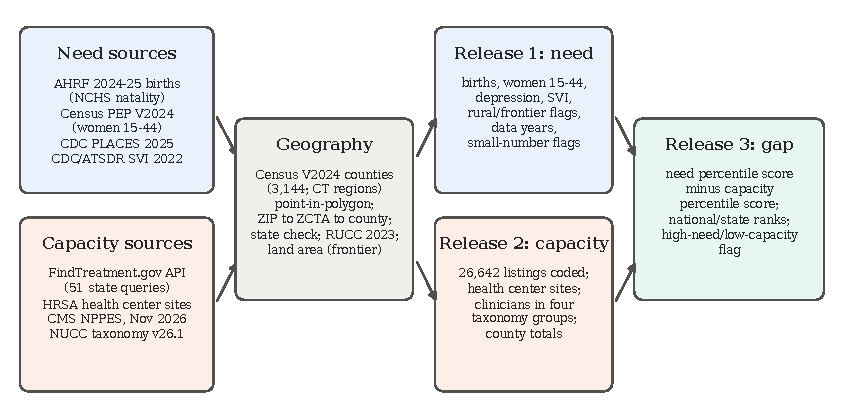
\includegraphics[width=0.92\textwidth]{figures/fig1_pipeline.pdf}
\caption{Build pipeline. Open need and capacity sources are harmonized to the Census Vintage 2024 county universe and released as three linked, versioned tables that share the five-digit county code.}
\label{fig:pipeline}
\end{figure*}

\subsection{Need measures}

\subsubsection{Births}
Annual births are the NCHS three-year average of resident births for 2021--2023 as published in the AHRF 2024--2025 (\texttt{births\_3yr\_avg\_23}). Where that value is unavailable, the Census estimate of births from July 2023 to June 2024 is used. Fallback applies to \NFallback\ counties: Connecticut's nine planning regions (AHRF reports NCHS births for the former counties) and \NFallbackSupp\ small counties where NCHS figures are suppressed. A source field and a years field accompany every value.

\subsubsection{Women of reproductive age}
Female residents aged 15--44 on 1~July 2024 come from the Vintage 2024 county characteristics file. The general fertility rate is $\mathrm{GFR}_i = 1000\,B_i/W_i$, where $B_i$ is births and $W_i$ is women aged 15--44 in county $i$.

\subsubsection{Depression and mental distress}
No open source reports perinatal depression for every county. We therefore use the model-based crude prevalence of adults ever told they have a depressive disorder from CDC PLACES, which applies multilevel regression and poststratification to BRFSS data~\cite{greenlund2022}. Age-adjusted prevalence and frequent mental distress are also carried. The 2025 PLACES release omits Kentucky and Pennsylvania; their \NPlacesPrior\ counties take values from the 2024 release (BRFSS 2022) and are flagged. One county (Loving, TX) has no PLACES value. The product $B_i \times p_i/100$, with $p_i$ the depression prevalence, is carried as a scale indicator and is explicitly not an estimate of perinatal cases.

\subsubsection{Social vulnerability}
The overall CDC/ATSDR Social Vulnerability Index percentile (0 least, 1 most vulnerable) and its four theme percentiles come from the 2022 county file~\cite{flanagan2011}.

\subsection{Capacity measures}

\subsubsection{Treatment listings}
FindTreatment.gov has no single bulk file. Its public locator API returns all listings in a state when queried with the state identifier documented in the developer guide~\cite{ftguide}. We issued 51 state queries without a service-type filter, so substance use (SA), mental health (MH), and opioid treatment program (OTP) listings were all returned; every query returned its full reported count (\FTRaw\ rows). Exact duplicates on name, street, ZIP, and type were removed (\FTUnique\ unique listings). Listings were placed in counties by point-in-polygon on the 2024 Census boundaries; listings without coordinates were placed by ZIP code (Sec.~\ref{sec:zip}). A state check re-placed by ZIP any listing whose coordinates fell in another state's county, which corrected \FTMismatch\ listings geocoded to same-named towns elsewhere. In total, \FTAssignedPct\% of listings were placed; \FTUnassigned\ (mostly P.O.~box ZIP codes) were not.

A listing is coded as a PPW program when its ``Special Programs/Groups Offered'' field contains ``Pregnant/postpartum women.'' This field is present only on SA listings: none of the \FTMH\ MH listings or \FTOTP\ OTP listings carries it. The facility capacity measure is therefore PPW \emph{substance use} treatment. Supporting flags record child care for clients' children, residential beds for children, Medicaid acceptance, and medications for opioid use disorder (MOUD).

\subsubsection{Health center sites}
From HRSA's file of health center service delivery and look-alike sites we count active, permanent service delivery sites, excluding administrative-only, seasonal, mobile, school, and correctional sites. Counties come from HRSA's county code, with one blank code placed by ZIP. In total, \HCSites\ sites in the 50 states and DC are counted, at \HCLocations\ distinct addresses; \HCUnplaced\ sites have no published address and cannot be placed.

\subsubsection{Clinicians}
From the November 2026 NPPES file (9.89 million records) we keep active individual providers (entity type 1) and assign each to one group by primary taxonomy (the code flagged primary, otherwise the first listed) at the primary practice ZIP (Table~\ref{tab:taxonomy}). Family physicians are reported but not added to obstetric capacity, because NPPES cannot show which of them provide obstetric care. Gynecology-only subspecialties, lay midwives, school-based and pastoral counselors, and child and adolescent psychiatry are excluded by design.

\begin{table}[!tbp]
\centering
\caption{Clinician groups by NUCC taxonomy (v26.1) and national counts placed in panel counties.}
\label{tab:taxonomy}
\footnotesize
\begin{tabular}{@{}p{1.6cm}p{4.6cm}r@{}}
\toprule
Group & Taxonomy (examples of codes) & $n$ \\
\midrule
Obstetric & OB/GYN 207V00000X; Obstetrics 207VX0000X; Maternal-fetal medicine 207VM0101X; Advanced practice midwife 367A00000X; Midwife 176B00000X; NP OB/GYN, women's health, perinatal; CNS women's health, perinatal & \OBTotal \\
BH prescriber & Psychiatry 2084P0800X; addiction psychiatry; psychosomatic medicine; addiction medicine (five boards); psychiatric/mental health NP 363LP0808X and CNS & \BHPTotal \\
BH therapist & Psychologist 103T*; clinical social worker 1041C0700X; counselor 101Y*, mental health, addiction, professional; marriage and family therapist 106H00000X & \BHTTotal \\
Family medicine & Family Medicine 207Q00000X (reported only) & \FMTotal \\
\bottomrule
\end{tabular}
\end{table}

\subsubsection{ZIP-to-county assignment}\label{sec:zip}
ZIPs are treated as ZIP Code Tabulation Areas (ZCTAs) and assigned to the county containing the largest share of the ZCTA's land area, using the 2020 Census relationship file. Because that file still uses Connecticut's former counties, Connecticut ZCTAs are assigned to planning regions by their 2024 Gazetteer interior point. ZIPs that are not ZCTAs remain unmatched (0.8\% of clinicians).

\subsection{Rural and frontier classification}
Counties with 2023 Rural-Urban Continuum Codes 4--9 (nonmetro) are rural~\cite{rucc}. Counties with fewer than six residents per square mile of land are frontier, the traditional population-density definition~\cite{ncfc}; frontier takes precedence. The resulting classes contain \NMetro\ metro, \NRural\ rural, and \NFrontier\ frontier counties.

\subsection{Need, capacity, and gap scores}
Let $x_{ik}$ be component $k$ for county $i$, and let $P(x_{ik})\in(0,100]$ be its national percentile rank (average ranks for ties, among counties with a value). Need components are adult depression prevalence and overall SVI; capacity components are, per 1,000 births, PPW SUD listings, behavioral health clinicians (prescribers plus therapists), obstetric clinicians, and health center sites. Then
\begin{align}
N_i &= \frac{1}{|K_N|}\sum_{k\in K_N} P(x_{ik}), \qquad C_i = \frac{1}{|K_C|}\sum_{k\in K_C} P(x_{ik}),\\
G_i &= N_i - C_i,\qquad G_i\in[-100,100].
\end{align}
A positive gap means a county ranks higher on need than on capacity. A county is flagged high need, low capacity (HNLC) when $N_i$ is in the top quartile and $C_i$ in the bottom quartile nationally. Counties with zero births (one county) receive no capacity score. Scores are relative ranks, not statements of absolute adequacy.

\subsection{Small numbers}
Following the CDC WONDER convention that rates based on 20 or fewer events are unreliable~\cite{wonder}, counties with fewer than 20 births (\NSmallBirths\ counties) are flagged, as are counties with one or two PPW listings. Section~\ref{sec:small} quantifies the resulting instability.

\subsection{Quality assurance, validation, and sensitivity analyses}
The pipeline writes a quality report with row counts at each stage, join and geocoding match rates, range checks, and named spot checks; the author verified Nevada values against his county maps and checked extreme and randomly selected counties against source websites. As external validation, NPPES obstetric clinicians and behavioral health prescribers were compared with AHRF counts of patient-care OB/GYN physicians and psychiatrists from the AMA Physician Masterfile (2023)~\cite{ahrf}. Eight alternative specifications of the gap score were compared with the baseline using Spearman correlation and the Jaccard overlap of HNLC sets (Table~\ref{tab:sens}).

\subsection{Statistical analysis and reproducibility}
We report counts, percentages, and medians, and use Kruskal--Wallis tests for differences in gap score across classes, a $\chi^2$ test for the absence of PPW programs by class, Spearman correlation for need--capacity association, and a Mann--Whitney test comparing need in counties with and without PPW programs. Analyses used Python 3.13 (pandas, GeoPandas, SciPy; figures in Matplotlib and seaborn). Numbered scripts rebuild every table from the public sources; every number in this paper is written to a statistics file and inserted into the manuscript programmatically.

\section{Results}

\subsection{Panel overview}
The panel covers \NCounties\ counties with \BirthsTotal\ births per year (Table~\ref{tab:rural}). Metro counties hold \PctBirthsMetro\% of births, rural counties \PctBirthsRural\%, and frontier counties \PctBirthsFrontier\%. Every county has births, women aged 15--44, SVI, RUCC, and land area; one lacks depression prevalence.

\begin{table}[!tbp]
\centering
\caption{County characteristics by rurality class. BH: behavioral health; PPW SUD: substance use treatment listing with a pregnant/postpartum women program. Scores are national percentile ranks (0--100).}
\label{tab:rural}
\scriptsize
\setlength{\tabcolsep}{3pt}
\resizebox{\columnwidth}{!}{\begin{tabular}{@{}lrrrr@{}}
\toprule
 & Metro & Rural & Frontier & All \\
\midrule
Counties & 1{,}164 & 1{,}563 & 417 & 3{,}144 \\
Births per year & 3{,}152{,}315 & 461{,}953 & 27{,}795 & 3{,}642{,}063 \\
Share of U.S. births (\%) & 86.6 & 12.7 & 0.8 & 100.0 \\
Women aged 15--44 & 59{,}278{,}483 & 7{,}695{,}613 & 428{,}770 & 67{,}402{,}866 \\
Adult depression, median (\%) & 23.2 & 23.5 & 20.9 & 23.0 \\
SVI overall, median & 0.47 & 0.56 & 0.34 & 0.50 \\
No PPW SUD program (\% of counties) & 35.1 & 65.5 & 86.6 & 57.0 \\
No behavioral prescriber (\%) & 11.2 & 30.3 & 72.4 & 28.8 \\
No obstetric clinician (\%) & 16.5 & 36.7 & 77.2 & 34.6 \\
No health center site (\%) & 18.6 & 30.6 & 65.9 & 30.8 \\
BH clinicians per 1,000 births, median & 219.5 & 127.8 & 70.0 & 155.4 \\
Obstetric clinicians per 1,000 births, median & 14.3 & 6.8 & 0.0 & 7.9 \\
Need score, median & 49.5 & 56.5 & 35.6 & 51.2 \\
Capacity score, median & 58.8 & 47.7 & 33.8 & 50.4 \\
Gap score, median & $-$7.9 & 6.9 & $-$1.6 & $-$0.1 \\
High need, low capacity (counties) & 23 & 72 & 12 & 107 \\
\bottomrule
\end{tabular}}
\end{table}

\subsection{Need}
Median adult depression prevalence was \DepMedMetro\% in metro, \DepMedRural\% in rural, and \DepMedFrontier\% in frontier counties; median SVI was \SVIMedMetro, \SVIMedRural, and \SVIMedFrontier. The two need components were nearly uncorrelated across counties (Spearman $\rho=\RhoDepSVI$), so they carry distinct information. Frontier counties therefore had the lowest median need score (\NeedMedFrontier, against \NeedMedRural\ rural and \NeedMedMetro\ metro), a pattern that reflects lower modelled depression and lower measured vulnerability in sparsely settled counties of the Great Plains and the West, rather than an absence of need.

\subsection{Capacity}
Placed listings comprised \FTPPWPlaced\ PPW SUD listings at \FTPPWLoc\ addresses, \ShareSAPPW\% of placed SA listings. Of PPW listings, \PPWMedicaid\% accepted Medicaid and \PPWMOUD\% offered MOUD, but only \PPWChildcare\% offered child care for clients' children and \PPWResbeds\% residential beds for children. The clinician inventory placed \OBTotal\ obstetric clinicians, \BHPTotal\ behavioral health prescribers, \BHTTotal\ behavioral health therapists, and \FMTotal\ family physicians in panel counties. Median behavioral health clinicians per 1,000 births fell from \BHPerKMetro\ in metro to \BHPerKRural\ in rural and \BHPerKFrontier\ in frontier counties; the median frontier county had no obstetric clinician (\OBPerKFrontier\ per 1,000 births).

\subsection{Counties without services}
\NNoPPW\ counties (\PctNoPPW\%) had no PPW SUD listing; they account for \BirthsNoPPW\ births a year, \PctBirthsNoPPW\% of the national total. Absence rose steeply with rurality (Fig.~\ref{fig:lacking}): \NoPPWMetro\% of metro, \NoPPWRural\% of rural, and \NoPPWFrontier\% of frontier counties ($\chi^2_2=\ChiSq$, $p\Chip$). In absolute terms, births in such counties were split nearly evenly between metro (\BirthsNoPPWMetro) and rural (\BirthsNoPPWRural) counties, with \BirthsNoPPWFrontier\ in frontier counties. \NNoBHP\ counties had no behavioral health prescriber, \NNoOB\ no obstetric clinician, and \NNoHC\ no counted health center site. \NNoAny\ counties, with \BirthsNoAny\ births a year, had none of a PPW SUD listing, a behavioral health prescriber, or an obstetric clinician.

\begin{figure}[!tbp]
\centering
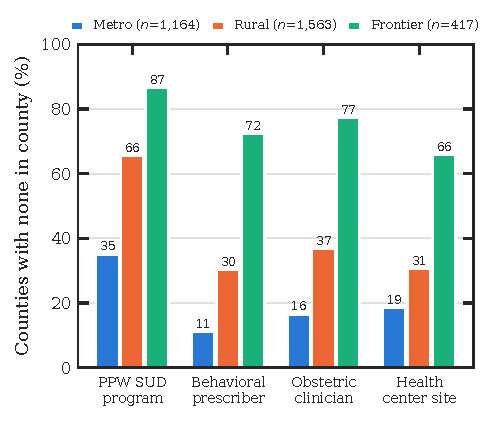
\includegraphics[width=\columnwidth]{figures/fig3_lacking_by_class.pdf}
\caption{Share of counties with no in-county capacity of each type, by rurality class. PPW SUD: substance use treatment listing with a pregnant/postpartum women program.}
\label{fig:lacking}
\end{figure}

\subsection{Need, capacity, and gap scores}
Need and capacity were weakly and positively associated (Spearman $\rho=\RhoNeedCap$, $p\RhoNeedCapp$; Fig.~\ref{fig:scatter}); each need component correlated with capacity at $\rho\approx\RhoDepCap$. Counties without a PPW listing had lower median need scores than counties with one (\NeedMedNoPPW\ vs.\ \NeedMedPPW; Mann--Whitney $p\MWp$), consistent with programs locating where measured need and population are larger. Gap scores differed by class (Kruskal--Wallis $H=\KWH$, $p\KWp$): the median was \GapMedMetro\ in metro, \GapMedRural\ in rural, and \GapMedFrontier\ in frontier counties.

The national map (Fig.~\ref{fig:map}) shows positive gaps concentrated across the lower Mississippi Valley and the Mid-South (state median gap highest in Louisiana and Tennessee), Alabama, Texas, Arkansas, Oklahoma, Kentucky, and Missouri, and negative gaps across the Northeast and Mid-Atlantic, Hawaii, Alaska, and Wyoming. \NHNLC\ counties met the HNLC definition: \HNLCRural\ rural, \HNLCFrontier\ frontier, and \HNLCMetro\ metro. They lay in \NStatesHNLC\ states, led by \HNLCStates. The 15 largest gaps (Table~\ref{tab:top}) all occurred in counties with at least 20 births, none of which had a PPW SUD listing.

\begin{figure*}[t]
\centering
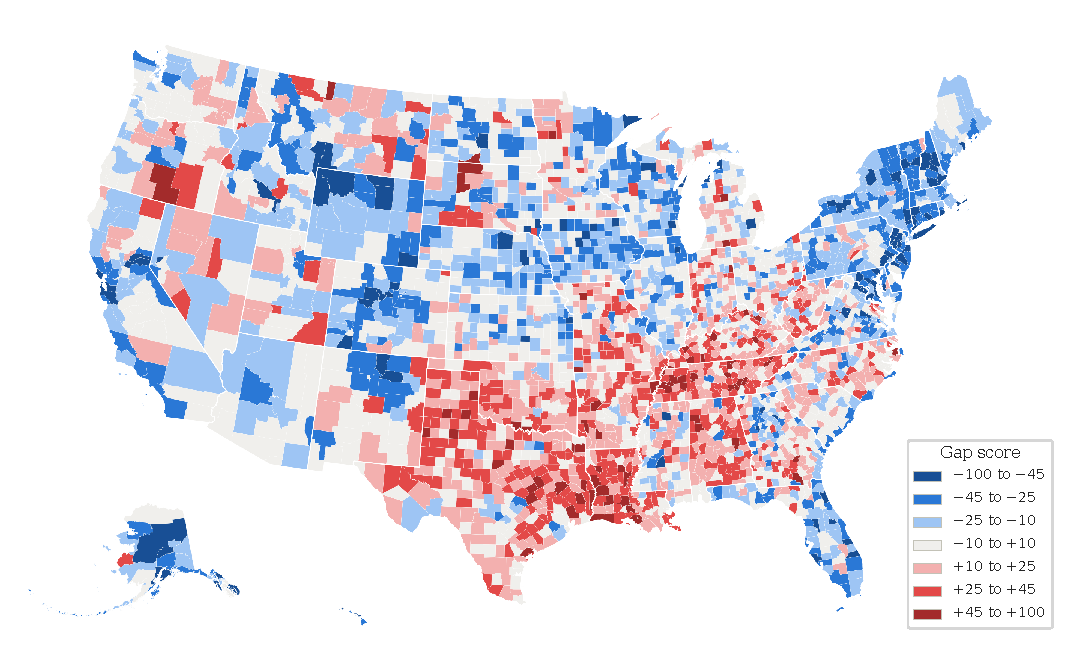
\includegraphics[width=0.94\textwidth]{figures/fig2_gap_map.pdf}
\caption{Gap score (need percentile minus capacity percentile) by county. Red: need ranks above capacity; blue: capacity ranks above need. Alaska and Hawaii are shown as insets, not to scale. Counties with fewer than 20 births are unstable (Sec.~\ref{sec:small}).}
\label{fig:map}
\end{figure*}

\begin{figure}[!tbp]
\centering
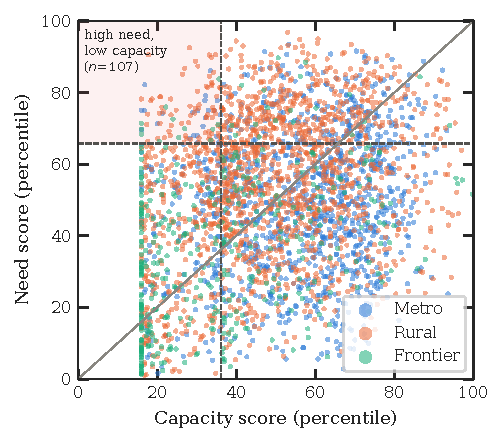
\includegraphics[width=\columnwidth]{figures/fig4_need_vs_capacity.pdf}
\caption{Need score against capacity score for each county. Dashed lines mark the top need quartile and bottom capacity quartile; the shaded corner holds high-need, low-capacity counties. The vertical band at the left edge is the tie among counties with no capacity of any measured type.}
\label{fig:scatter}
\end{figure}

\begin{table*}[t]
\centering
\caption{The 15 counties with the largest gap scores. Dep.: adult depression prevalence; PPW: PPW SUD listings; BH: behavioral health clinicians; OB: obstetric clinicians. Need and gap are percentile-based scores.}
\label{tab:top}
\small
\begin{tabular}{@{}rllrrrrrrrr@{}}
\toprule
\# & County & Class & Births & Dep.\,\% & SVI & PPW & BH & OB & Need & Gap \\
\midrule
1 & Mahnomen, MN & rural & 77 & 26.6 & 0.96 & 0 & 2 & 0 & 90.6 & +72.8 \\
2 & Crockett, TN & metro & 164 & 27.9 & 0.72 & 0 & 2 & 0 & 82.2 & +65.3 \\
3 & Lauderdale, TN & rural & 285 & 27.9 & 0.92 & 0 & 9 & 0 & 92.5 & +64.3 \\
4 & Jefferson, OK & rural & 68 & 25.4 & 0.81 & 0 & 0 & 0 & 78.2 & +62.2 \\
5 & McDonald, MO & rural & 326 & 26.5 & 0.89 & 0 & 9 & 0 & 86.8 & +59.8 \\
6 & Newton, TX & rural & 113 & 25.0 & 0.85 & 0 & 4 & 0 & 78.2 & +59.5 \\
7 & Jack, TX & rural & 91 & 24.0 & 0.94 & 0 & 3 & 0 & 77.7 & +59.3 \\
8 & DeKalb, TN & rural & 250 & 30.1 & 0.80 & 0 & 10 & 0 & 88.8 & +59.1 \\
9 & Hopewell city, VA & metro & 321 & 24.1 & 0.88 & 0 & 0 & 0 & 75.1 & +59.1 \\
10 & Rhea, TN & rural & 384 & 30.2 & 0.72 & 0 & 12 & 0 & 85.1 & +58.7 \\
11 & Sequatchie, TN & metro & 181 & 31.3 & 0.50 & 0 & 2 & 0 & 75.0 & +58.2 \\
12 & Henderson, TN & rural & 307 & 29.0 & 0.63 & 0 & 17 & 0 & 78.8 & +58.1 \\
13 & Tyler, TX & rural & 195 & 24.3 & 0.93 & 0 & 11 & 0 & 78.8 & +58.0 \\
14 & St. Mary, LA & rural & 605 & 27.3 & 0.91 & 0 & 20 & 2 & 90.5 & +57.3 \\
15 & Haywood, TN & rural & 193 & 26.7 & 0.89 & 0 & 6 & 0 & 87.4 & +57.1 \\
\bottomrule
\end{tabular}
\end{table*}

\subsection{State variation}
States differed widely in the share of births occurring in counties without a PPW SUD listing (Fig.~\ref{fig:states}). The highest shares were in \TopStates; in \ZeroStates\ every birth occurred in a county with at least one such listing. PPW SUD listings per 10,000 births ranged from \StateMinPPW\ (\StateMinPPWst) to \StateMaxPPW\ (\StateMaxPPWst), with a state median of \StateMedPPW.

\begin{figure}[!tbp]
\centering
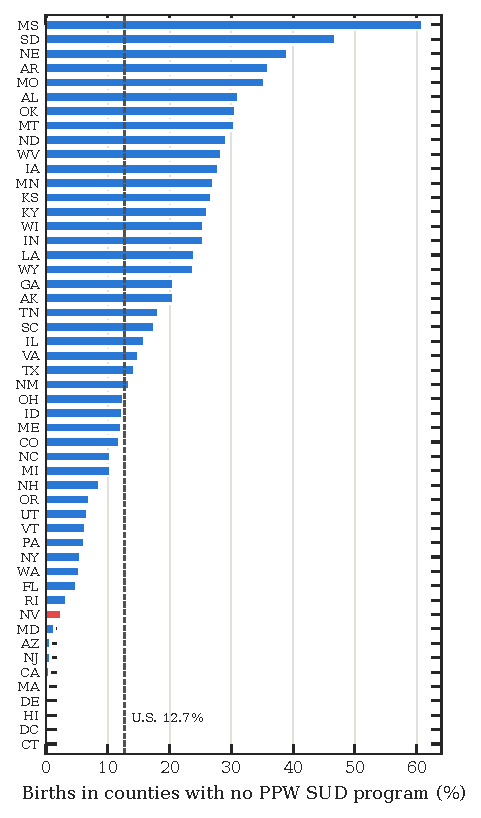
\includegraphics[width=0.94\columnwidth]{figures/fig5_states.pdf}
\caption{Share of each state's births occurring in counties with no PPW SUD listing. Dashed line: national share. Nevada is highlighted.}
\label{fig:states}
\end{figure}

\subsection{External validation of clinician counts}
Across \ValN\ matched counties, NPPES obstetric clinicians tracked AHRF OB/GYN physician counts closely (log-scale Pearson $r=\ValROB$, Spearman $\rho=\ValRhoOB$), as did behavioral health prescribers and AHRF psychiatrists ($r=\ValRPsy$, $\rho=\ValRhoPsy$; Fig.~\ref{fig:val}). NPPES totals were higher (\ValSumOBN\ vs.\ \ValSumOBA\ obstetric; \ValSumPsyN\ vs.\ \ValSumPsyA\ prescriber), as expected because the NPPES groups include midwives and nurse practitioners and because NPPES records registrations rather than verified active practice. The two sources agreed on whether a county had any such clinician in \ValZeroOB\% (obstetric) and \ValZeroPsy\% (prescriber) of counties.

\begin{figure*}[t]
\centering
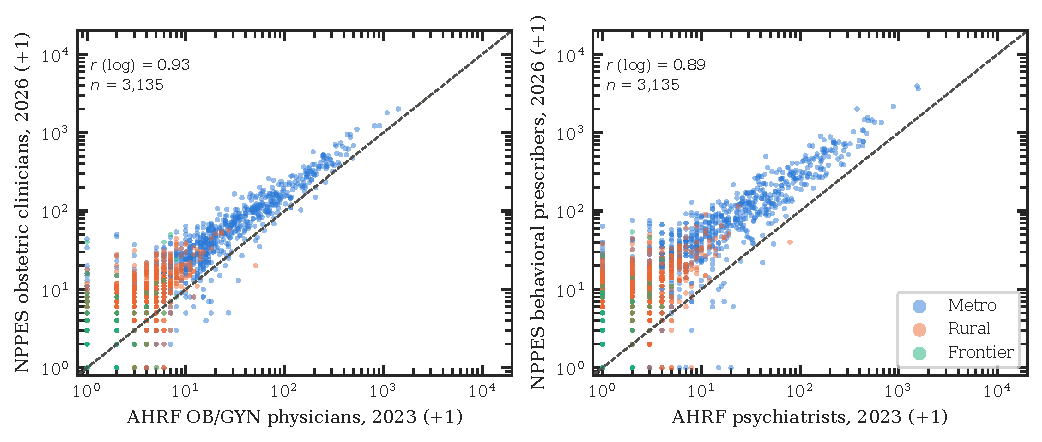
\includegraphics[width=0.86\textwidth]{figures/fig6_validation.pdf}
\caption{External validation. County counts of NPPES obstetric clinicians against AHRF (AMA Physician Masterfile) OB/GYN physicians (left), and of NPPES behavioral health prescribers against AHRF psychiatrists (right). Axes are log scale after adding one; the dashed line is equality.}
\label{fig:val}
\end{figure*}

\subsection{Small-county instability}\label{sec:small}
Per-birth ratios are unstable where births are few, and the instability runs in both directions (Fig.~\ref{fig:small}). Most of the \NSmallBirths\ counties with fewer than 20 births score low on capacity because they have no measured capacity at all (median capacity score \CapMedSmall, against \CapMedBig\ for the \NBirthsBig\ counties with more than 2,000 births). A few score very high because a single clinician or site becomes a large rate: Storey County, Nevada, with 18 births a year and two obstetric clinicians, has one of the most negative gaps in the country. Expressing capacity per 1,000 women aged 15--44 does not resolve this (gap-rank correlation with baseline $\rho=\SensWomenRho$; Storey's gap moves only to $-\SensWomenStorey$). Leaving counties with fewer than 20 births unranked removes the artifact while changing the HNLC set modestly (Jaccard \SensUnrankedJac). The released panel ranks every county and flags small counties; users ranking counties against each other should exclude or separately report flagged counties.

\begin{figure}[!tbp]
\centering
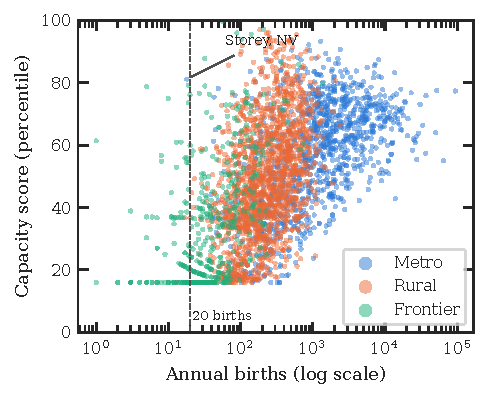
\includegraphics[width=\columnwidth]{figures/fig7_small_counties.pdf}
\caption{Capacity score against annual births (log scale). Left of the dashed line (fewer than 20 births), scores cluster at the floor or jump high on a single clinician.}
\label{fig:small}
\end{figure}

\subsection{Sensitivity analyses}
Gap rankings were robust to every alternative (Table~\ref{tab:sens}, Fig.~\ref{fig:sens}): Spearman correlations with the baseline were at least \SensRhoMin. Counting health centers or PPW programs by address, rather than by site or listing, changed almost nothing. The HNLC set, a threshold on two quartiles, was more sensitive: overlap with the baseline set fell to a Jaccard index of \SensJacMin\ when mental health listings were added to capacity, and was also reduced when prescribers alone represented behavioral health or when frequent mental distress was added to need. Policy use of the HNLC flag should therefore state the specification.

\begin{table}[!tbp]
\centering
\caption{Sensitivity of the gap score. $\rho$: Spearman correlation with baseline gap ranks (among counties scored in both). HNLC $n$: high-need, low-capacity counties; overlap and Jaccard against the baseline set of \NHNLC.}
\label{tab:sens}
\scriptsize
\setlength{\tabcolsep}{3pt}
\begin{tabular}{@{}lrrrr@{}}
\toprule
Specification & $\rho$ & HNLC $n$ & Overlap & Jaccard \\
\midrule
Baseline & 1.000 & 107 & 107 & 1.00 \\
Capacity per 1,000 women aged 15--44 & 0.994 & 104 & 99 & 0.88 \\
Counties with $<$20 births unranked & $>$0.999 & 110 & 101 & 0.87 \\
Health centers counted by address & $>$0.999 & 106 & 104 & 0.95 \\
PPW programs counted by address & $>$0.999 & 107 & 107 & 1.00 \\
Age-adjusted depression & 0.989 & 115 & 99 & 0.80 \\
Need adds frequent mental distress & 0.975 & 122 & 93 & 0.68 \\
Capacity adds MH listings & 0.973 & 104 & 78 & 0.59 \\
Behavioral prescribers only & 0.973 & 110 & 85 & 0.64 \\
\bottomrule
\end{tabular}
\end{table}

\begin{figure*}[t]
\centering
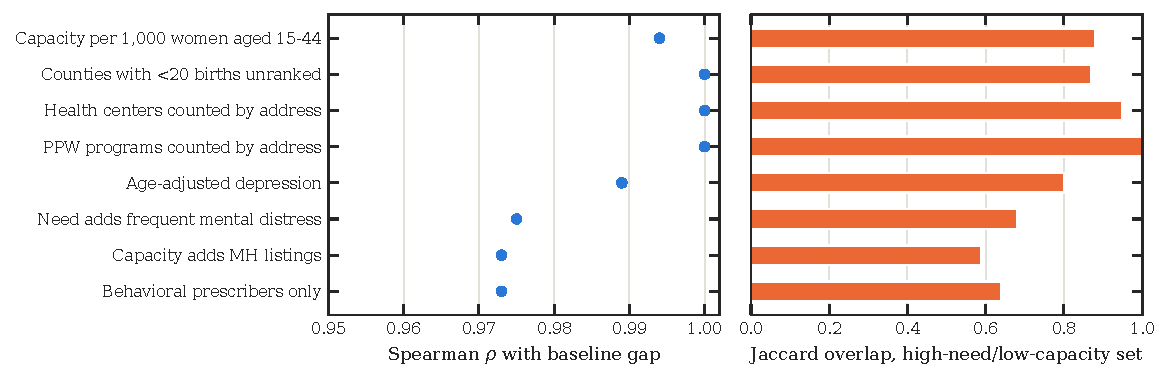
\includegraphics[width=0.9\textwidth]{figures/fig9_sensitivity.pdf}
\caption{Sensitivity analyses. Left: rank agreement of alternative gap scores with the baseline. Right: agreement of the alternative high-need, low-capacity sets with the baseline set.}
\label{fig:sens}
\end{figure*}

\subsection{Nevada}
Nevada illustrates the national pattern at state scale (Table~\ref{tab:nv}, Fig.~\ref{fig:nv}). Of its 17 counties, \NVFrontier\ are frontier under the density definition. All \NVPPW\ Nevada PPW SUD listings are in seven counties; \NVNoPPW\ counties have none, although they account for only \NVPctBirthsNoPPW\% of the state's \NVBirths\ births, because Clark and Washoe counties hold \NVCWBirths\% of births and \NVCWPPW\% of PPW listings. \NVNoOB\ counties have no obstetric clinician and \NVNoBHP\ no behavioral health prescriber. The largest Nevada gaps are in Esmeralda and Eureka, both with fewer than 20 births, followed by Lincoln, Mineral, Humboldt, Pershing, and Lander; Storey's strongly negative gap is the small-number artifact described above. The author's prior Nevada mapping was used to check these values.

\begin{figure}[!tbp]
\centering
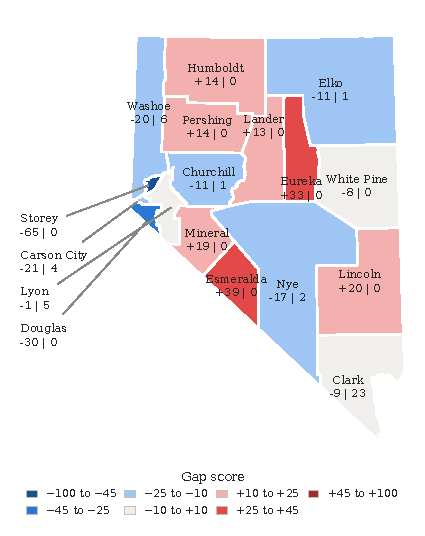
\includegraphics[width=0.95\columnwidth]{figures/fig8_nevada.pdf}
\caption{Nevada gap scores. Labels give the gap score and the number of PPW SUD listings. Esmeralda, Eureka, and Storey have fewer than 20 births a year.}
\label{fig:nv}
\end{figure}

\begin{table}[!tbp]
\centering
\caption{Nevada county values. HC: health center sites; other abbreviations as in Table~\ref{tab:top}. $^\dagger$Fewer than 20 births.}
\label{tab:nv}
\scriptsize
\setlength{\tabcolsep}{2.6pt}
\begin{tabular}{@{}llrrrrrrrr@{}}
\toprule
County & Class & Births & Dep.\,\% & SVI & PPW & HC & OB & BH & Gap \\
\midrule
Carson City & metro & 512 & 21.4 & 0.85 & 4 & 1 & 17 & 248 & $-$20.6 \\
Churchill & frontier & 280 & 22.0 & 0.63 & 1 & 0 & 4 & 104 & $-$11.0 \\
Clark & metro & 24,629 & 20.3 & 0.86 & 23 & 38 & 414 & 7,126 & $-$8.8 \\
Douglas & rural & 323 & 18.9 & 0.21 & 0 & 0 & 4 & 92 & $-$30.0 \\
Elko & frontier & 676 & 21.5 & 0.62 & 1 & 4 & 7 & 77 & $-$10.9 \\
Esmeralda$^\dagger$ & frontier & 2 & 20.2 & 0.91 & 0 & 0 & 0 & 0 & +38.8 \\
Eureka$^\dagger$ & frontier & 18 & 23.5 & 0.43 & 0 & 0 & 0 & 0 & +33.2 \\
Humboldt & frontier & 204 & 21.7 & 0.62 & 0 & 0 & 2 & 23 & +14.1 \\
Lander & frontier & 61 & 22.8 & 0.58 & 0 & 1 & 0 & 4 & +12.6 \\
Lincoln & frontier & 52 & 21.2 & 0.57 & 0 & 0 & 0 & 5 & +19.9 \\
Lyon & metro & 622 & 21.4 & 0.56 & 5 & 0 & 1 & 62 & $-$1.2 \\
Mineral & frontier & 33 & 22.3 & 0.55 & 0 & 0 & 0 & 6 & +19.1 \\
Nye & frontier & 382 & 21.0 & 0.80 & 2 & 3 & 3 & 98 & $-$17.4 \\
Pershing & frontier & 42 & 19.6 & 0.68 & 0 & 0 & 0 & 6 & +13.5 \\
Storey$^\dagger$ & metro & 18 & 19.7 & 0.18 & 0 & 1 & 2 & 21 & $-$64.8 \\
Washoe & metro & 4,949 & 21.1 & 0.70 & 6 & 12 & 99 & 2,204 & $-$19.8 \\
White Pine & frontier & 85 & 21.5 & 0.25 & 0 & 0 & 0 & 37 & $-$7.6 \\
\bottomrule
\end{tabular}
\end{table}

\FloatBarrier
\section{Discussion}

\subsection{Principal findings}
This panel shows that specialized substance use treatment for pregnant and postpartum women is absent from most U.S. counties, overwhelmingly so in rural and frontier counties, and that about one in eight births occurs in a county without such a program. Because need and capacity are only weakly related across counties, a relative gap score identifies a distinct set of places where measured need is high and every measured form of capacity is thin. Those places cluster in the rural South, Kentucky and Tennessee, and the southern Plains, and most are rural rather than frontier. Frontier counties lack nearly every form of in-county capacity, but their modelled need is also lower, so their median gap is close to zero; for them, the absence flags and travel to care, rather than the gap score, are the relevant measures.

\subsection{Relation to prior work}
Our finding that PPW programs are present in a minority of SA listings (\ShareSAPPW\%) is consistent with national facility surveys reporting that about a quarter to a third of facilities offer perinatal programming~\cite{macpac2020,lombardi2025}. Low availability of child care and residential beds for children among PPW programs echoes earlier survey analyses~\cite{meinhofer2020,lombardi2025}. The steep rural gradient in behavioral health prescribers and obstetric clinicians agrees with NPPES-based workforce studies~\cite{andrilla2018} and with documented losses of rural obstetric services~\cite{hung2017,kozhimannil2018,mod2024}. The contribution here is not a new count of any single resource but a single, open county table that holds need and several forms of capacity together, with their data years and flags, so that others can recombine them.

\subsection{Implications}
For state agencies, the absence flags identify counties where a pregnant woman screened positive for substance use disorder has no specialized program in her county, and the HNLC flag identifies counties where adding referral and treatment capacity would address both high need and low supply. Where in-county programs are unlikely to be sustainable, models that extend specialist reach to frontline obstetric clinicians, such as perinatal psychiatry access programs~\cite{byatt2016}, and acceptance of pregnant patients by existing MOUD prescribers~\cite{patrick2020} are natural levers. Because the PPW field exists only for substance use listings, a direct recommendation to SAMHSA is to collect a comparable perinatal program item from mental health facilities; until then, perinatal mental health capacity cannot be mapped from open facility data.

\subsection{Limitations}
First, need is measured with stand-ins: adult depression prevalence for all adults and social vulnerability rank counties sensibly but do not measure perinatal depression, anxiety, or substance use directly. Second, the facility measure covers substance use treatment only and rests on self-reported directory entries that may be out of date. Third, NPPES counts are registrations at a primary practice address; they do not establish active practice, Medicaid participation, acceptance of pregnant patients, full-time effort, secondary sites, or telehealth across county lines. Fourth, county lines are not care boundaries; a county without a program may be near one across the line. Fifth, small counties are unstable (Sec.~\ref{sec:small}). Sixth, scores are relative ranks. Seventh, data years differ across measures, from births in 2021--2023 to listings in November 2026, and each column records its year. Eighth, about 0.3\% of listings, 0.8\% of clinicians, and \HCUnplaced\ health center sites could not be placed, and ZIP codes spanning counties are assigned to the county with most of their land. Ninth, home visiting, certified community behavioral health clinics, and women's set-aside programs, all part of the author's Nevada mapping, lack open national site lists suitable for this version. Finally, the territories are excluded.

\subsection{Future work}
Planned versions will add travel-time capacity within 30 and 60 minutes, smoothed or shrinkage estimates for small counties, state-level perinatal depression context from PRAMS, and annual refreshes released under the same concept DOI.

\section{Conclusions}
An open, reproducible county panel built only from federal public data can show where perinatal behavioral health need outpaces treatment capacity across the United States. Most counties, and most rural and frontier counties, have no specialized substance use program for pregnant and postpartum women, and a distinct set of mostly rural counties combines high need with low capacity on every measured dimension. We release the panel, code, codebook, coding rules, and provenance so that agencies and researchers can verify, extend, and act on it.

\section*{Data and code availability}
\noindent The panel is released in three versioned parts (need measures; capacity inventory; gap scores) with codebook, coding rules, limitations, quality reports, and provenance logs. Code and data: \url{https://github.com/memesobum/perinatal-bh-panel}; each release is archived on Zenodo with its own DOI, listed in the repository README. All inputs are public and are re-downloaded by the pipeline. Data and documents are licensed CC~BY~4.0 and code MIT.

\section*{Author contributions}
\noindent M.A.E.: conceptualization, methodology, data curation, validation, formal analysis, visualization, writing (original draft, review and editing).

\section*{Use of AI tools}
\noindent Claude (Anthropic) assisted with code, data handling, and drafting. The author made every measurement decision, verified results against source data and his Nevada county maps, and takes responsibility for the content.

\section*{Funding, competing interests, and ethics}
\noindent This work received no funding. The author declares no competing interests. The study used only publicly available, aggregate, or public-registry data; released clinician data are aggregated to ZIP and county counts without names or identifiers. It did not involve human subjects research.

\begin{thebibliography}{99}

\bibitem{cdc_mmrc2020} Centers for Disease Control and Prevention. Pregnancy-related deaths: data from maternal mortality review committees in 38 U.S. states, 2020. Atlanta, GA: CDC; 2024. \url{https://www.cdc.gov/maternal-mortality/php/data-research/index.html}

\bibitem{bauman2020} B.~L. Bauman, J.~Y. Ko, S.~Cox, D.~V. D'Angelo, L.~Warner, S.~Folger, H.~D. Tevendale, K.~C. Coy, L.~Harrison, and W.~D. Barfield. Vital signs: postpartum depressive symptoms and provider discussions about perinatal depression---United States, 2018. \emph{MMWR Morb. Mortal. Wkly. Rep.}, 69(19):575--581, 2020. doi:10.15585/mmwr.mm6919a2

\bibitem{luca2020} D.~L. Luca, C.~Margiotta, C.~Staatz, E.~Garlow, A.~Christensen, and K.~Zivin. Financial toll of untreated perinatal mood and anxiety disorders among 2017 births in the United States. \emph{Am. J. Public Health}, 110(6):888--896, 2020. doi:10.2105/AJPH.2020.305619

\bibitem{acog_cpg4} American College of Obstetricians and Gynecologists. Screening and diagnosis of mental health conditions during pregnancy and postpartum: ACOG Clinical Practice Guideline No.~4. \emph{Obstet. Gynecol.}, 141(6):1232--1261, 2023. doi:10.1097/AOG.0000000000005200

\bibitem{byatt2016} N.~Byatt, K.~Biebel, T.~A. Moore Simas, B.~Sarvet, M.~Ravech, J.~Allison, and J.~Straus. Improving perinatal depression care: the Massachusetts Child Psychiatry Access Project for Moms. \emph{Gen. Hosp. Psychiatry}, 40:12--17, 2016. doi:10.1016/j.genhosppsych.2016.03.002

\bibitem{andrilla2018} C.~H.~A. Andrilla, D.~G. Patterson, L.~A. Garberson, C.~Coulthard, and E.~H. Larson. Geographic variation in the supply of selected behavioral health providers. \emph{Am. J. Prev. Med.}, 54(6 Suppl 3):S199--S207, 2018. doi:10.1016/j.amepre.2018.01.004

\bibitem{hung2017} P.~Hung, C.~E. Henning-Smith, M.~M. Casey, and K.~B. Kozhimannil. Access to obstetric services in rural counties still declining, with 9 percent losing services, 2004--14. \emph{Health Aff.}, 36(9):1663--1671, 2017.

\bibitem{kozhimannil2018} K.~B. Kozhimannil, P.~Hung, C.~Henning-Smith, M.~M. Casey, and S.~Prasad. Association between loss of hospital-based obstetric services and birth outcomes in rural counties in the United States. \emph{JAMA}, 319(12):1239--1247, 2018. doi:10.1001/jama.2018.1830

\bibitem{mod2024} A.~Stoneburner, R.~Lucas, J.~Fontenot, C.~Brigance, E.~Jones, and A.~L. DeMaria. Nowhere to go: maternity care deserts across the US (Report No.~4). March of Dimes; 2024.

\bibitem{macpac2020} Medicaid and CHIP Payment and Access Commission. Access to treatment for pregnant women with a substance use disorder and infants with neonatal abstinence syndrome. Commission meeting presentation, January 2020.

\bibitem{meinhofer2020} A.~Meinhofer, J.~M. Hinde, and M.~M. Ali. Substance use disorder treatment services for pregnant and postpartum women in residential and outpatient settings. \emph{J. Subst. Abuse Treat.}, 110:9--17, 2020. doi:10.1016/j.jsat.2019.12.005

\bibitem{lombardi2025} B.~N. Lombardi, A.~B. Parisi, H.~Newton, and B.~M. Lombardi. Characteristics of substance use disorder and mental health disorder treatment facilities with perinatal programs. \emph{J. Subst. Use Addict. Treat.}, 209722, 2025.

\bibitem{patrick2020} S.~W. Patrick, M.~R. Richards, W.~D. Dupont, et~al. Association of pregnancy and insurance status with treatment access for opioid use disorder. \emph{JAMA Netw. Open}, 3(8):e2013456, 2020. doi:10.1001/jamanetworkopen.2020.13456

\bibitem{greenlund2022} K.~J. Greenlund, H.~Lu, Y.~Wang, K.~A. Matthews, J.~M. LeClercq, B.~Lee, and S.~A. Carlson. PLACES: local data for better health. \emph{Prev. Chronic Dis.}, 19:210459, 2022. doi:10.5888/pcd19.210459

\bibitem{flanagan2011} B.~E. Flanagan, E.~W. Gregory, E.~J. Hallisey, J.~L. Heitgerd, and B.~Lewis. A social vulnerability index for disaster management. \emph{J. Homel. Secur. Emerg. Manag.}, 8(1):3, 2011. doi:10.2202/1547-7355.1792

\bibitem{ahrf} Health Resources and Services Administration. Area Health Resources Files, 2024--2025 county release and technical documentation. \url{https://data.hrsa.gov/data/download?data=AHRF}

\bibitem{pep} U.S. Census Bureau. County population totals and characteristics, Vintage 2024. \url{https://www2.census.gov/programs-surveys/popest/datasets/2020-2024/counties/}

\bibitem{rucc} U.S. Department of Agriculture, Economic Research Service. Rural-Urban Continuum Codes, 2023. \url{https://www.ers.usda.gov/data-products/rural-urban-continuum-codes}

\bibitem{census_geo} U.S. Census Bureau. 2024 Gazetteer files; 2024 cartographic boundary files; 2020 ZCTA to county relationship file. \url{https://www.census.gov/geographies/reference-files.html}

\bibitem{ftguide} Substance Abuse and Mental Health Services Administration. FindTreatment.gov API documentation, version 1.12, 17 August 2026. \url{https://findtreatment.gov/assets/FindTreatment-Developer-Guide.pdf}

\bibitem{hrsa_sites} Health Resources and Services Administration. Health center service delivery and look-alike sites, HRSA Data Warehouse. \url{https://data.hrsa.gov/data/download}

\bibitem{nppes} Centers for Medicare \& Medicaid Services. NPPES downloadable file, version 2, November 2026. \url{https://download.cms.gov/nppes/NPI_Files.html}

\bibitem{nucc} National Uniform Claim Committee. Health Care Provider Taxonomy code set, version 26.1. \url{https://www.nucc.org}

\bibitem{ncfc} National Center for Frontier Communities. Frontier definitions. \url{https://frontierus.org}

\bibitem{wonder} Centers for Disease Control and Prevention. CDC WONDER natality data documentation: reliability of rates. \url{https://wonder.cdc.gov/wonder/help/natality.html}

\end{thebibliography}

\end{document}
